\section{Darstellung im Dreidimensionalen}
\todo[color=red]{Kasten für Formel hinzufügen}
\todo[color=red]{Zusammenfassung-Kasten hinzufügen}
\todo[color=red]{Signalwörter-Kasten hinzufügen}
Sollen Punkte, Ebenen oder Geraden in ein Koordinatensystem gezeichnet werden, so sollten wir uns zunächst noch einmal Gedanken darüber machen, wie man die Achsen einträgt. Die y-Achse wird nach rechts hin aufgetragen, die z-Achse nach oben hin. Bei der x-Achse, welche nach links vorne gezeichnet wird (\(45^{\circ}\) zur y-Achse), besteht die Besonderheit, dass eine Längeneinheit nur halb so lang gezeichnet wird. Das ist auch bei der Einteilung der x-Achse zu beachten!

\subsection{Gerade}
\todo[color=red]{Kasten für Formel hinzufügen}
\todo[color=red]{Zusammenfassung-Kasten hinzufügen}
\todo[color=red]{Signalwörter-Kasten hinzufügen}
Auch wenn es selten vorkommt, werden wir zur Sicherheit erwähnen, wie man sie einzeichnet. Nehmt dazu den Stützvektor und zeichnet ihn ein. Ebenso wie einen zweiten Vektor auf der Gerade (den bekommt ihr, indem ihr zum Beispiel s=1 setzt). Dann verbindet ihr die Punkte mit einer Linie und schon habt ihr die Gerade. 

\subsection{Ebenen (Spurpunkte \& -geraden)}
\todo[color=red]{Kasten für Formel hinzufügen}
\todo[color=red]{Zusammenfassung-Kasten hinzufügen}
\todo[color=red]{Signalwörter-Kasten hinzufügen}

    \begin{figure}[h]
    \centering
    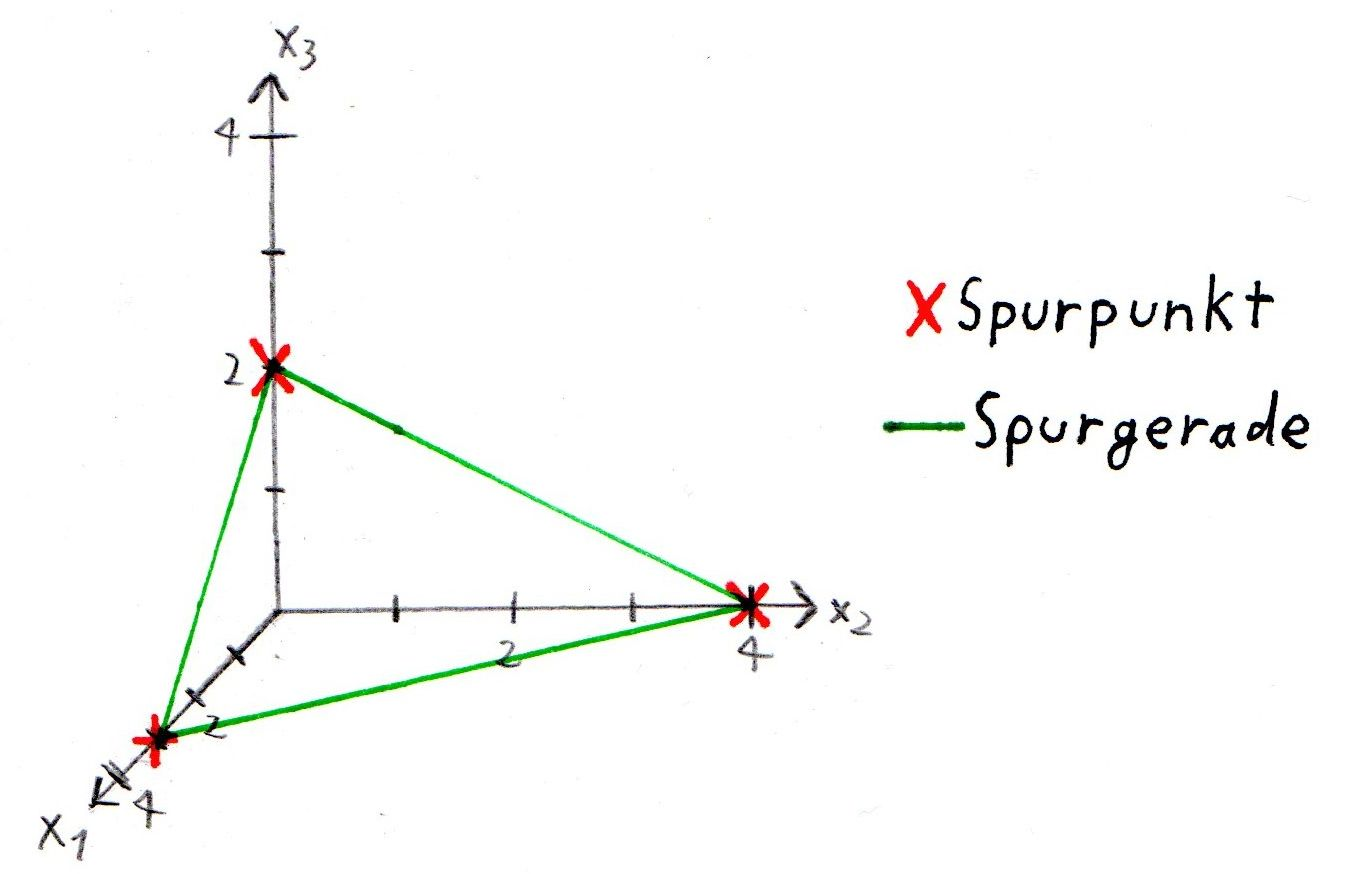
\includegraphics[scale=0.2]{Images/Spurpunkte.jpeg}
    \caption{Spurpunkte und Geraden einer Ebene}
    \end{figure}

Um Ebenen darzustellen, nimmt man sich Spurpunkte bzw. -geraden zur Hilfe. Wenn nicht anders verlangt, raten wir zu den Spurpunkten. Das sind die Punkte, in denen die Ebene die Achsen schneidet. Man berechnet sie einfach, indem man (für das Schneiden mit der x-Achse) y=z=0 setzt und erhält so einen Wert für x. Mit den anderen Punkten, die man natürlich synchron dazu berechnet, spannt sich dann eine Ebene auf.\\
Die Spurgeraden sind Geraden, die durch jeweils zwei Spurpunkte gehen. Diese benötigt man lediglich bei Ebenen, die in der Parameterform dargestellt sind. Dazu setzt man bei \(\vec{x}\) einfach eine Koordinate 0 und berechnet dann die Parameter in dieser Zeile.

\subsection{einfache geometrische Formen im Raum}
\todo[color=red]{Kasten für Formel hinzufügen}
\todo[color=red]{Zusammenfassung-Kasten hinzufügen}
\todo[color=red]{Signalwörter-Kasten hinzufügen}
Jegliche Formen im Raum darzustellen, ist recht leicht. Hierzu setzt ihr einfach alle angegebenen Punkte ins Koordinatensystem ein und verbindet die Punkte (überlegt euch, welche Punkte überhaupt verbunden werden müssen, bei einem Quadrat ABCD ist es nicht sinnvoll, AC und BD zu verbinden).
